%----------------------- Wydruk dwustronny ---------------
%\documentclass[12pt,twoside,a4paper]{book} % 
%----------------------- Wydruk jednostronny ---------------
\documentclass[12pt,oneside,a4paper]{book} % jednostronnego

\usepackage{polski}
\usepackage[utf8]{inputenc} %opcja dla edytorów kodujących polskie znaki w utf8
%\usepackage[cp1250]{inputenc} %opcja dla edytorów kodujących polskie znaki w windows-1250
\usepackage{lmodern}
\usepackage{indentfirst}
\usepackage[protrusion=false]{microtype}
\DisableLigatures{encoding = *, family = * }
\usepackage{fancyhdr}
\usepackage{pstricks,graphicx}
\usepackage{amssymb}
\usepackage{float}

\usepackage{pdflscape}
\usepackage{diagbox}

%---------------Zbiory liczbowe
\newcommand{\R}{\mathbb{R}}
\newcommand{\N}{\mathbb{N}}
\newcommand{\K}{\mathbb{K}}
\newcommand{\C}{\mathcal{C}}
\newcommand{\p}{\mathcal{P}}
%------------kwantyfikatory--------------
\newcommand{\fal}{\mbox{{\Large $\forall\,$}}}
\newcommand{\ext}{\mbox{{\Large $\exists\,$}}}
%------------------definicje środowisk-----------------
\usepackage{theorem}
\theoremstyle{break}
\theorembodyfont{\it}
\newtheorem{twr}{Twierdzenie}[chapter]
\newtheorem{lem}{Lemat}[chapter]
\theorembodyfont{\rm}
\newtheorem{defi}{Definicja}[chapter]
\newtheorem{wni}{Wniosek}[chapter]
\newtheorem{prz}{Przykład}[chapter]
\newenvironment{dowod}{\par\vspace{0.1cm}\par{ \sc Dowód.}}{\hfill $\blacksquare$\par\vspace{0.4cm}\par}
% ----------ustawienia wymiarow strony
\usepackage{geometry}

\newgeometry{tmargin=2.5cm, bmargin=2.5cm, headheight=14.5pt, inner=3cm, outer=2.5cm} 

\linespread{1.1} %-zmiana interlinii


\fancypagestyle{mylandscape}{
\fancyhf{} %Clears the header/footer
\fancyfoot{% Footer
\makebox[\textwidth][r]{% Right
  \rlap{\hspace{.75cm}% Push out of margin by \footskip
    \smash{% Remove vertical height
      \raisebox{4.87in}{% Raise vertically
        \rotatebox{90}{\thepage}}}}}}% Rotate counter-clockwise
\renewcommand{\headrulewidth}{0pt}% No header rule
\renewcommand{\footrulewidth}{0pt}% No footer rule
}

%---------------- Normalne środowiska --------------------
\usepackage{amsmath}

%----------nagłowki i żywa pagina ------------
\pagestyle{fancy} 
%--------------- Wydruk dwustronny
%\cfoot[]{} 
%\lhead[{\scriptsize{\it \thepage}}]{}
%\chead[{\scriptsize\leftmark}]{{\scriptsize \rightmark}}
%\rhead[]{{\scriptsize{\it \thepage}}}
%--------------- Wydruk jednostronny
\fancyhead[C]{} 
\fancyfoot[C]{\thepage}
\fancyhead[L]{\scriptsize\leftmark}
\fancyhead[R]{\scriptsize\rightmark}

\renewcommand{\chaptermark}[1]{%
\markboth{\MakeUppercase{%
\chaptername}\ \thechapter.%
\ #1}{}}

\usepackage[most]{tcolorbox}
\let\includegraphicsold\includegraphics
\newcommand{\includegraphicsborder}[2][]{\tcbox{\includegraphicsold[#1]{#2}}}

\renewcommand{\sectionmark}[1]{\markright{\thesection.\ #1}}

\usepackage[hidelinks]{hyperref}

\usepackage{graphics}
\graphicspath{ {images/} }

\usepackage{listings}

\renewcommand{\lstlistlistingname}{Spis listingów}
\renewcommand{\lstlistingname}{Listing}

\lstset{
  basicstyle=\footnotesize
}

\usepackage{booktabs}

\newcommand\tabularhead[2]{
  \begin{table}[ht]
    \label{#2}
    \caption{#1}
    \begin{tabular}{|p{0.35\linewidth}|p{0.6\linewidth}|}
    \hline
    \textbf{#1}\\
    \hline
}
\newcommand\addrow[2]{#1 &#2\\ \hline}

\newcommand\addmulrow[2]{ \begin{minipage}[t][][t]{2.5cm}#1\end{minipage}
   &\begin{minipage}[t][][t]{8cm}
    \begin{enumerate} #2   \end{enumerate}
    \end{minipage}\\ }

\newenvironment{usecase}{\tabularhead}
{\hline\end{tabular}\end{table}}



%-----------------właściwa część pracy-----------------
\begin{document}
\thispagestyle{empty}
\begin{center}
  \Large
  \bf{UNIWERSYTET ŚLĄSKI}\\
  \bf{\sf{WYDZIAŁ NAUK ŚCISŁYCH I TECHNICZNYCH}}\\[25mm]
  \large

  \bf{Porównanie klasyfikatorów z RSES}\\[35mm]

  Sprawozdanie\\
  z przedmiotu\\
  Eksploracja Danych\\[25mm]
\end{center}
\begin{flushright}
  \large
  Autorzy:\\
  Kacper Małachowski\\
\end{flushright}
\vspace*{\fill}
\begin{center}
  Informatyka II Stopnia\\
  Lato 2023/2024\\
  I rok, grupa 3\\[25mm]
\end{center}

\chapter*{Źródło danych}

Dane pochodzą z repozytorium uniwersytetu kalifornijskiego, gdzie znajdują się pod nazwą "Room Occupancy Estimation".
Stworzone zostały w ramach badań: Adarsh Pal Singh, Vivek Jain, Sachin Chaudhari, Frank Alexander Kraemer, Stefan Werner and Vishal Garg, "Machine Learning-Based Occupancy Estimation Using Multivariate Sensor Nodes," in 2018 IEEE Globecom Workshops (GC Wkshps), 2018.

\subsection*{Opis atrybutów}

\begin{itemize}
  \item Date - Pominięty w eksploracji - Data pomiaru z czujników.
  \item Time - Pominięty w eksploracji - Czas pomiaru z czujników z dokładnością do sekund.
  \item S1\_Temp - Odczyt z czujnika temperatury umieszczonego przy biurku nr 1, podany w stopniach celsjusza.
  \item S2\_Temp - Odczyt z czujnika temperatury umieszczonego przy biurku nr 2, podany w stopniach celsjusza.
  \item S3\_Temp - Odczyt z czujnika temperatury umieszczonego przy biurku nr 3, podany w stopniach celsjusza.
  \item S4\_Temp - Odczyt z czujnika temperatury umieszczonego przy biurku nr 4, podany w stopniach celsjusza.
  \item S1\_Light - Odczyt z czujnika światła umieszczonego przy biurku nr 1, podany w luxach.
  \item S2\_Light - Odczyt z czujnika światła umieszczonego przy biurku nr 2, podany w luxach.
  \item S3\_Light - Odczyt z czujnika światła umieszczonego przy biurku nr 3, podany w luxach.
  \item S4\_Light - Odczyt z czujnika światła umieszczonego przy biurku nr 4, podany w luxach.
  \item S1\_Sound - Odczyt z przetwornika analogowo-cyfrowego podłączonego do wyjścia wzmacniacza mikrofonu, wyrażony w woltach. Czujnik ten umieszczony jest przy biurku nr 1.
  \item S2\_Sound - Odczyt z przetwornika analogowo-cyfrowego podłączonego do wyjścia wzmacniacza mikrofonu, wyrażony w woltach. Czujnik ten umieszczony jest przy biurku nr 2.
  \item S3\_Sound - Odczyt z przetwornika analogowo-cyfrowego podłączonego do wyjścia wzmacniacza mikrofonu, wyrażony w woltach. Czujnik ten umieszczony jest przy biurku nr 3.
  \item S4\_Sound - Odczyt z przetwornika analogowo-cyfrowego podłączonego do wyjścia wzmacniacza mikrofonu, wyrażony w woltach. Czujnik ten umieszczony jest przy biurku nr 4.
  \item S5\_CO2 - Odczyt z detektora CO2, umieszczonego na środku pokoju, wyrażony w cząsteczkach na milion.
  \item S5\_CO2\_Slope - Zmiana stężenia CO2 w pomieszczeniu z detektora umieszczonego na środku pomieszczenia.
  \item S6\_PIR - Wartość prawda-fałsz wskazująca na wykrycie ruchu przez czujnik umieszczony nad drzwiami.
  \item S7\_PIR - Wartość prawda-fałsz wskazująca na wykrycie ruchu przez czujnik umieszczony na ścianie na przeciwko drzwi.
\end{itemize}

\chapter*{Projekt w RSES}

Poniżej przedstawiono zdjęcia projektu w programie RSES.
Projekt 0 odpowiedzialny jest za wczytanie i dyskretyzacje danych.
\begin{figure}[H]
  \centering
  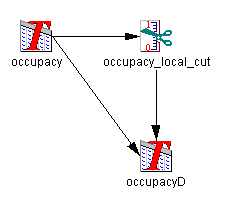
\includegraphics[width=1\textwidth]{project0.png}
\end{figure}

Poniżej przedstawiono przykładowy projekt odpowiedzialny za eksploracje danych, pozostałe projekty wyglądają tak samo.

\begin{figure}[H]
  \centering
  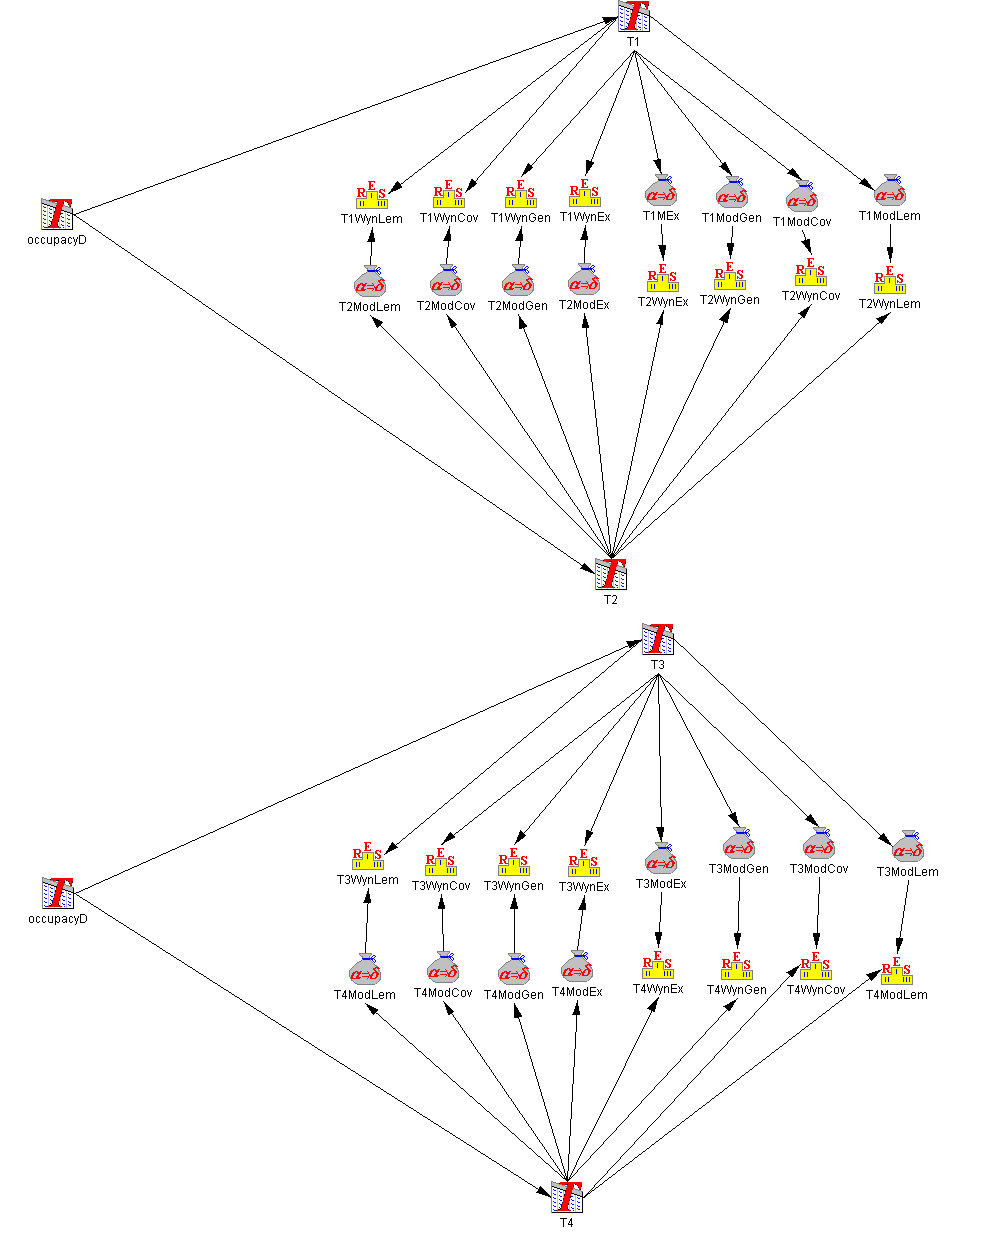
\includegraphics[width=1\textwidth]{project1.png}
\end{figure}

\subsection*{Opis składowych projektu}

Projekt podzielono na dwa rodzaje projektów, jeden odpowiedzialny za dyskretyzacje danych oraz drugi za uzyskiwanie wyników.
Cały projekt składa się łacznie z sześciu projektów, jednego odpowiedzialnego za dyskretyzacje i pięciu zawierających po dwa podziały danych.

\subsubsection*{Dyskretyzacja}

W projekcie zero, dane wczytane z pliku .tab utworoznego na oryginalnego pliku .csv podlegają dyskretyzacji, która wykonywana jest przy pomocy cięć utworzonych metodą lokalną z pominięciem atrybutów typu symbolic.

Tak przetworzone dane zapisano wp liku occupacyD.tab, który posłużył jako wejście dla pozotałych projektów.

\subsubsection*{Proces eksploracji}

Każdy projekt z wynikami składa się z dwóch tabel z danymi wczytanymi z pliku occupacyD.tab, które zostały podzielone w sposób losowy na dwie kolejne tabele każda służące za biory treningowe i testowe.

W ten sposób w każdym projekcie uzyskano cztery tabele wejściowe dla algorytmów oraz dwa podziały.

Następnie z każdej tabel (T1, T2, T3 i T4) wyprowadzono zbiory reguł czterama różnymi algorytmami.

\begin{itemize}
  \item Wyczerpujący (Ex) - algorytm nie posiada parametrów.
  \item Genetyczny (Gen) - z paramterem prędkości ustawionym na duzą oraz parametrem reduktów o wartosci 10.
  \item Pokryciowy (Cov) - z parametrem pokrycia na 0.9.
  \item LEM2 (Lem) - z paramterem pokrycia na 0.9.
\end{itemize}

Następnie skorzystano z przeciwnej tabeli (np. dla tabeli 1, tabelą przeciwną jest tabela 2) do przetestowania skuteczności tak utworzonych reguł. Zbiory reguł nazwano w formacie "[nazwa tabeli treningowej]Mod[skrót algorytmu]", na przykład dla zestawu tabel 4 i 3, gdzie to tabela 4 jest zbiorem treningowym algorytmu wyczerpującego zbiór reguł ma nazwę "T4ModEx". Podobnie nazwano wyniki poszczególnych testów tj. "[nazwa tabeli testowej]Wyn[skrót algorytmu]", więc dla powyższego przykładu wyniki nazywają się "T3WynEx".

Nazewnictwo to zastosowano we wszystkich projektach, poza projektem zerowym.

\begin{landscape}
\thispagestyle{mylandscape}
\chapter*{Wyniki}

W poniższej tabeli przedstawiono wyniki dla poszczególnych klasyfikatorów. Wyniki wyrażone są jako iloczyn dokładności i pokrycia zapisany jako procent.

\begin{table}[H]
  \resizebox{1.5\textwidth}{!}{
  \begin{tabular}{|c|c|c|c|c|c|c|c|c|c|c|c|c|c|c|c|c|c|c|c|c|c|c|}
  \hline
  \backslashbox{Klasyfikator}{Iteracja}  & 1 & 2 & 3 & 4 & 5 & 6 & 7 & 8 & 9 & 10 & 11 & 12 & 13 & 14 & 15 & 16 & 17 & 18 & 19 & 20 & Średnia \\ \hline
   Wyczerpujący  & 99.6\% & 99.4\% & 99.6\% & 99.5\% & 99.5\% & 99.6\% & 99.6\% & 99.5\% & 99.5\% & 99.7\% & 99.5\% & 99.4\% & 99.3\% & 99.6\% & 99.6\% & 99.4\% & 99.3\% & 99.7\% & 99.7\% & 99.6\% & 99.53\% \\ \hline
   Genetyczny    & 99.6\% & 99.5\% & 99.6\% & 99.6\% & 99.5\% & 99.6\% & 99.6\% & 99.5\% & 99.6\% & 99.7\% & 99.5\% & 99.5\% & 99.4\% & 99.6\% & 99.6\% & 99.4\% & 99.3\% & 99.7\% & 99.7\% & 99.6\% & 99.56\% \\ \hline
   Pokryciowy    & 83.4\% & 84.5\% & 84.1\% & 86.8\% & 83.9\% & 85.6\% & 83.8\% & 85.1\% & 57.8\% & 84.3\% & 84.5\% & 83.6\% & 85.3\% & 57.9\% & 83.6\% & 58.8\% & 81.6\% & 57.6\% & 83.5\% & 84.4\% & 79.01\% \\ \hline
   LEM2          & 92.5\% & 93.2\% & 92.8\% & 93.1\% & 92.1\% & 93.0\% & 93.2\% & 92.6\% & 92.3\% & 93.2\% & 93.0\% & 92.1\% & 92.2\% & 93.3\% & 92.3\% & 92.7\% & 92.5\% & 92.8\% & 92.4\% & 93.0\% & 92.72\% \\ \hline
  \end{tabular}}
  \end{table}

\end{landscape}

\chapter*{Wnioski}

Najlepszy wynik spośród wszystkich trzech projektów odnotowano na drugiej ścieżce w projekcie nr 4, było to 99.56\%. To jest poprawa o 0.03 punkta procentowego względem drugiej ścieżki w drugim projekcie.

Pokazuje to, że algorytm genetyczny może poprawić wyniki klasyfikacji w stosunku do bardziej zaawansowanych algorytmów takich jak k-NN zastosowany w projekcie drugim.

Ponadto dobry algorytm dyskretyzacji użyty w programie RSES pozwala wyciągnąć z danych więcej szczegółów.

Natomiast wyniki ostatniego projektu pokazują jak dużą rolę w eksploracji danych odgrywa odpowiedni podział danych, różnica rzędu 20 punktów procentowych przy jedynej różnicy polegającej na innym podziale danych pokazuje to jednoznacznie.

Reasumując, podczas eksploracji danych istotnym jest nie tylko samo przygotowanie danych czy dobór klasyfikatora, ale również odpowiedni dobór podziału na zbiory treningowe i testowe, zapewniający jak największe zróżnicowanie danych w zbiorze treningowym

\end{document}